\usepackage[T1]{fontenc}% Mustervorlage für Abschlussarbeiten am LS DBIS
% Author: Alexander Stahl (stahlale@b-tu.de)
% Zuletzt aktualisiert am 10.02.2022

% Hinweis: Die Daten zur Arbeit speichern Sie in der Datei "data.tex".

% Diese Datei enthält Einstellungen und Paketimporte.
% Zur besseren Ordnung sollten Sie weitere Einstellungen bzw. Importe dieser Datei anfügen.

% Paketimporte
\documentclass[11pt,a4paper,german]{scrreprt}
\usepackage[utf8]{inputenc}  % Encoding
\usepackage{babel}  % Unterstützung verschiedener Sprachen
\usepackage{graphicx}  % Einbindung von Grafiken
\usepackage{amsmath}  % Verschiedene Symbole
\usepackage{tabularx}
\usepackage{ragged2e}
\usepackage{amssymb}  % Verschiedene Symbole
\usepackage{latexsym}  % Verschiedene Symbole
\usepackage{booktabs}  % Schönere Tabellen
\usepackage{multicol}  % Flexiblere Tabellen
\usepackage[printonlyused]{acronym}  % Abkürzungsverwaltung
\usepackage{hyperref}  % Klickbare URLs, Titel und PDF-Metadaten
\usepackage{lipsum}  % Platzhaltertext (kann entfernt werden)
\usepackage[backend=bibtex,style=ieee]{biblatex}  % Moderne Literaturverwaltung
\usepackage{tikz} % Graphen zeichnen

\usetikzlibrary{positioning,shapes,shadows,arrows}

% Einstellungen
\hypersetup{
    colorlinks,
    citecolor=black,
    filecolor=black,
    linkcolor=black,
    urlcolor=black
}

\makeatletter

\newcommand\frontmatter{
	\cleardoublepage
	\pagenumbering{roman}}

\newcommand\mainmatter{
	\cleardoublepage
	\pagenumbering{arabic}}

\newcommand\backmatter{
  \if@openright
    \cleardoublepage
  \else
    \clearpage
  \fi
   }

\usepackage{listings}
\usepackage{xcolor}

\colorlet{punct}{red!60!black}
\definecolor{background}{HTML}{EEEEEE}
\definecolor{delim}{RGB}{20,105,176}
\colorlet{numb}{magenta!60!black}

\lstdefinelanguage{json}{
    basicstyle=\normalfont\ttfamily,
    numbers=left,
    numberstyle=\scriptsize,
    stepnumber=1,
    numbersep=8pt,
    showstringspaces=false,
    breaklines=true,
    frame=lines,
    backgroundcolor=\color{background},
    literate=
    *{0}{{{\color{numb}0}}}{1}
        {1}{{{\color{numb}1}}}{1}
        {2}{{{\color{numb}2}}}{1}
        {3}{{{\color{numb}3}}}{1}
        {4}{{{\color{numb}4}}}{1}
        {5}{{{\color{numb}5}}}{1}
        {6}{{{\color{numb}6}}}{1}
        {7}{{{\color{numb}7}}}{1}
        {8}{{{\color{numb}8}}}{1}
        {9}{{{\color{numb}9}}}{1}
        {:}{{{\color{punct}{:}}}}{1}
        {,}{{{\color{punct}{,}}}}{1}
        {\{}{{{\color{delim}{\{}}}}{1}
        {\}}{{{\color{delim}{\}}}}}{1}
        {[}{{{\color{delim}{[}}}}{1}
        {]}{{{\color{delim}{]}}}}{1},
}

% GraphQL-Syntax-Hervorhebung
\lstdefinelanguage{GraphQL}{
    keywords={query, mutation, subscription, fragment, on, true, false, null},
    sensitive=true,
    comment=[l]{\#},
    morecomment=[s]{/*}{*/},
    string=[b]",
    morestring=[b]',
    literate=
        {<=}{{$\leq$}}2
        {>=}{{$\geq$}}2
        {!=}{{$\neq$}}2
        {==}{{$=$}}2
        {&&}{{\&\&}}2
        {||}{{$\mid\mid$}}2
        {...}{{$\ldots$}}2
%{_}{{$\lambda$}}1
        {\\\\}{{\char`\\\char`\\}}1
        {\\n}{{\char`\\n}}1
        {\\t}{{\char`\\t}}1
        {\\u2028}{{\char`\\u2028}}1
        {\\u2029}{{\char`\\u2029}}1
        {\\v}{{\char`\\v}}1
        {\\b}{{\char`\\b}}1
        {\\r}{{\char`\\r}}1
        {\\f}{{\char`\\f}}1,
}

% Einstellungen für den Code-Stil
\lstset{
    basicstyle=\ttfamily,
    keywordstyle=\color{blue},
    commentstyle=\color{gray},
    stringstyle=\color{orange},
    numbers=left,
    numberstyle=\scriptsize\color{gray},
    frame=single,
    breaklines=true,
    showstringspaces=false,
    captionpos=b,
}


\lstdefinelanguage{Python}{
    keywords={False, None, True, and, as, assert, break, class, continue, def, del, elif, else, except, finally, for, from, global, if, import, in, is, lambda, nonlocal, not, or, pass, raise, return, try, while, with, yield},
    keywordstyle=\color{blue}\bfseries,
    identifierstyle=\color{black},
    commentstyle=\color{gray}\itshape,
    stringstyle=\color{orange},
    morestring=[b]',
    morestring=[b]",
    morecomment=[s]{"""}{"""},
    morecomment=[l]{\#},
    morecomment=[s]{'''}{'''},
    sensitive=true,
    showstringspaces=false,
}


\definecolor{backcolour}{rgb}{0.95,0.95,0.92}
\definecolor{codegreen}{rgb}{0,0.6,0}
\definecolor{codegray}{rgb}{0.5,0.5,0.5}
\definecolor{codepurple}{rgb}{0.58,0,0.82}
\definecolor{codered}{rgb}{0.64,0.08,0.08}

\lstdefinelanguage{javascript}{
    keywords={const, let, break, case, catch, continue, debugger, default, delete, do, else, finally, for, function, if, in, instanceof, new, return, switch, this, throw, try, typeof, var, void, while, with, yield, import, export, async, await},
    keywordstyle=\color{blue}\bfseries,
    ndkeywords={class, enum, interface, extends, super, public, static, getter, setter},
    ndkeywordstyle=\color{codered}\bfseries,
    identifierstyle=\color{black},
    sensitive=false,
    comment=[l]{//},
    morecomment=[s]{/*}{*/},
    commentstyle=\color{codegreen}\ttfamily,
    stringstyle=\color{codepurple}\ttfamily,
    morestring=[b]',
    morestring=[b]"
}

% Laden der Literaturdaten
\addbibresource{quellen.bib}
\newtheorem{definition}{Definition}
\newtheorem{example}{Beispiel}
% Definition der Dokumentendaten
% Zur besseren Kapselung wurde die Eingabe Ihrer Daten in diese Datei ausgelagert.
% Bitte einfach ausfüllen.

\newcommand{\TitelDeutsch}{Integrationstesten von GraphQL mittels Prime-Path Abdeckung} % Hier zentral angeben
\newcommand{\TitelEnglisch}{Integration testing of GraphQL using Prime-Path Coverage} % Übersetzten Titel auch angeben
\newcommand{\ArbeitsTyp}{Masterarbeit} % unzutreffendes hier löschen
\newcommand{\AuthorName}{Tom Lorenz} % Hier ändern
\newcommand{\MatrikelNr}{3711679}
\newcommand{\Studiengang}{Informatik M. Sc.}
\newcommand{\DatumThemenausgabe}{16.05.2023}
\newcommand{\DatumAbgabe}{31.8.2023}
\newcommand{\BetreuerEins}{Prof. Dr. rer. nat. Leen Lambers}
\newcommand{\BetreuerZwei}{Prof. Dr. rer. nat. Gerd Wagner} % Bitte immer akademische Titel angeben
\newcommand{\GutachterEins}{M. Sc. Lucas Sakizloglou} % Bitte immer akademische Titel angeben
  % In dieser Datei die Daten der Arbeit eingeben.

\titlehead{{Brandenburgische Technische Universität Cottbus-Senftenberg\\ Institut für Informatik\\ Fachgebiet Praktische Informatik/Softwaresystemtechnik}}
\subject{Masterarbeit\\ \vspace{0.5cm}
\includegraphics[width=0.5\textwidth]{img/btu-logo}}
\title{\TitelDeutsch \\ {\normalsize \TitelEnglisch}}
\author{\AuthorName \\ MatrikelNr.: \MatrikelNr \\Studiengang: \Studiengang}
\date{\textit{Datum der Themenausgabe: \DatumThemenausgabe} \\ \textit{Datum der Abgabe: \DatumAbgabe}}
\publishers{ Betreuer 1: \BetreuerEins \\ Betreuer 2: \BetreuerZwei \\ Gutachter: \GutachterEins}

\hypersetup{pdfauthor={\AuthorName}}
\hypersetup{pdftitle={\TitelDeutsch}}

\tikzstyle{abstract}=[rectangle, draw=black, rounded corners, fill=blue!40, drop shadow,
text centered, anchor=north, text=white, text width=3cm]
\tikzstyle{comment}=[rectangle, draw=black, rounded corners, fill=green, drop shadow,
text centered, anchor=north, text=white, text width=3cm]
\tikzstyle{myarrow}=[->, >=open triangle 90, thick]
\tikzstyle{line}=[-, thick] % Header beinhaltet alle Einstellungen und Pakete. Bei Bedarf erweitern.

\begin{document}
  \frontmatter % kennzeichnet den vorderen Teil der Arbeit
  \maketitle % Titelseite generieren

  % Eidesstattliche Erklärung über Selbstständigkeit
  \section*{Eidesstattliche Erklärung}
Der Verfasser erklärt, dass er die vorliegende Arbeit selbständig, ohne fremde Hilfe und ohne Benutzung anderer als der angegebenen Hilfsmittel angefertigt hat.
Die aus fremden Quellen (einschließlich elektronischer Quellen) direkt oder indirekt übernommenen Gedanken sind ausnahmslos als solche kenntlich gemacht.
Wörtlich und inhaltlich verwendete Quellen wurden entsprechend den anerkannten Regeln wissenschaftlichen Arbeitens zitiert.
Die Arbeit ist nicht in gleicher oder vergleichbarer Form (auch nicht auszugsweise) im Rahmen einer anderen Prüfung bei einer anderen Hochschule vorgelegt oder publiziert worden.
Der Verfasser erklärt sich zudem damit einverstanden, dass die Arbeit mit Hilfe eines Plagiatserkennungsdienstes auf enthaltene Plagiate überprüft wird.

\vspace{2cm}

\noindent
\begin{tabular}{lcl}
  .................................... & \hspace{.4\textwidth} & ....................................\\
  Ort, Datum &  & Unterschrift

\end{tabular}


  % Automatische Generierung verschiedener Verzeichnisse
  % Inhaltsverzeichnis
  \addcontentsline{toc}{section}{Table of Contents}
  \tableofcontents
  \mainmatter
  % Es folgt der Haupttext der Arbeit. Passen Sie die Überschriften der Kapitel entsprechend an.
  % Beachten Sie, dass die hier angegebene Gliederung nur ein Vorschlag ist.
  % Außerdem wird empfohlen, jedes Kapitel in eine eigene Datei auszulagern und hier nur mittels \input einzubinden.
  %! Author = Tom
%! Date = 07.12.2022
\section{Abstract}

Mit zunehmender Popularität von GraphQL ist es wichtig auch die Qualität von GraphQL-Api's zu testen.
Aktuell gibt es aber noch eine Lücke an Testtools für GraphQL-Apis. Im Paper "Automatic Property-based Testing of
GraphQL APIs" (Quelle hinzufügen) wurde sich mit einem automatischen Testverfahren für GraphQL-API's beschäftigt.
Allerdings bietet diese Arbeit ein Verbesserungspotential, welches in dieser Arbeit untersucht und implementiert werden soll.
Im konkreten handelt es sich bei dem automatischen Testverfahren um ein Verfahren, dass ein GraphQL-Schema aufgrund seiner
Eigenschaften aufspaltet und Testet. Hierbei wird zwar Rücksicht auf die Graphstruktur genommen allerdings werden spezifische
Grapheigenschaften nicht ausgenutzt um die Tests zu verbessern. Ziel dieser Arbeit ist es, das Domänenwissen für Graphen zu nutzen
um eine automatische Testgenerierung zu verbessern und algorithmisch beweisbar eine ideale Abdeckung mit Tests zu erreichen.




  %! Author = Tom
%! Date = 07.12.2022
\chapter{Einleitung}

In diesem Kapitel wird an das Thema und die Motivation dieser Arbeit herangeführt.
Außerdem wird definiert, welche Ziele diese Arbeit erreichen soll und eine grobe Übersicht über die
Kapitelstruktur gegeben.

\section{Motivation}

Mit einer steigenden Nutzung von GraphQL wird es immer wichtiger, geeignete Tests für GraphQL-API's zu entwickeln damit eine
gute Softwarequalität sichergestellt werden kann.
Idealerweise können diese Testtools solche API's automatisch testen,
so wie es für REST-API's schon umgesetzt wurde.
Die Struktur von GraphQL erlaubt allerdings zyklische Strukturen
und ermöglicht somit ein potentenziell unendlich großen Testraum.
In dem Paper " Automatic Property-based Testing of GraphQL-API's " (hier Quelle) wurde versucht ein solches
automatisches Testtool zu entwickeln. Ergebniss der Arbeit war hierbei ein Prototyp der in der Lage ist
eine GraphQL-Schnittstelle zu testen allerdings mit zwei technischen Einschränkungen.
Die erste technische Limitierung liegt in der Lösung des potentiell unendlichen Testraumes, hierbei
wird ein Rekursionslimit festgelegt, dass die maximale Pfadlänge festlegt und somit für einen endlichen Suchraum sorgt.
Diese Arbeit soll zeigen, dass die erste technische Limitierung lösbar ist durch einen spezifischen Algorithmus.
Eine zweite Limitierung ist die Auswertung der Tests. GraphQL liefert eine stark typisierte Antwort, die vorhersehbar
durch die Schemadefinition ist. Im Testtool wird allerdings nur die Typsierung getestet. Dies bedeutet, dass eine gewisse
Anzahl an false-positives existieren können geschuldet daraus, dass nur der Typ eines Objektes getestet wird, jedoch nicht
seine Exakten Attribute.

Der allgemeine Ablauf des bestehenden Tools ist wie folgt:
\begin{center}
    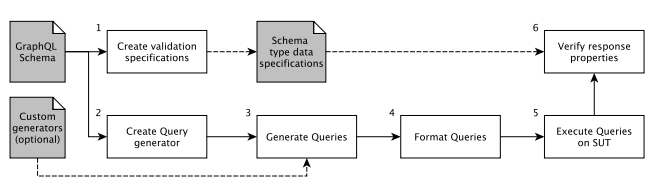
\includegraphics[width=\textwidth,height=\textheight,keepaspectratio]{content/einleitung/toolchain}
\end{center}

Verbesserungen in dieser Arbeit sind insbesondere in den Punkten 2 und 6 (6 wenn genug Zeit) geplant.

\begin{description}
    \item[Create Query Generator (Punkt 2)] Kapitel Testgenerierung
    \item[Verify response properties (Punkt 6)] Kapitel Testauswertung
\end{description}

\subsection{Testgenerierung}

Der bisherige Ansatz der Testgenerierung ist eine zufallsbasierte Suche.
Hierbei wird ein GraphQL-Schema geladen und nach dem Query-Type gefragt.
Der Query-Type definiert alle erlaubten Anfragen an die API.
Das Ergebnis einer jeden Anfrage ist (ein Knoten) / (eine Liste von Knoten).
Jeder Knoten kann dann verwandte Knoten haben.
Eben diese werden dann mit zufallsbasierter Suche abgefragt, jedoch nur bis zu einer bestimmten Pfadlänge die
durch das Rekursionslimit festgelegt ist, eben um unendliche Suchräume zu vermeiden.
Nun ist offensichtlich, dass es durchaus auch Pfade geben kann, die länger
als das Rekursionslimit sind und somit nicht vom Testtool berücksichtig werden.
Im Sinne einer guten Testcoverage wollen wir aber möglichst
jede Funktion mit Tests überdecken, somit erreicht die bisherige Methode leider nicht eine zufriedenstellende Lösung im Sinne
der Testcoverage.
Diese Arbeit soll die bisherige Methode verbessern indem Schritt 2, der Query-Generator, verbessert wird mit einem
endlichen Algorithmus der Graphen jeder Größe und Struktur zuverlässig abdeckt. Hierfür müssen verschiedene Überdeckungskriterien
erst definiert werden, allerdings sei schon zu sagen, die hier vorgestellte Methode hat als Ziel, das jede Kante und jeder
Knoten des Graphens hierdurch mit mindestens einem Test abgedeckt werden, sodass wir eine erhebliche Verbesserung in der
Zuverlässigkeit der Testcoverage erlangen.

\subsection{Testauswertung}


Die Auswertung der Tests nach " Automatic Property-based Testing of GraphQL-API's " erfolgt durch einen Typabgleich von Query und Response.
Eine Validierung der Response wird zeitgleich mit dem erstellen der Querys erledigt. Hierdurch folgt die Limitierung, dass das Testtool
aus dem GraphQL-Schema wissen kann, welchen Typ eine Antwort hat, allerdings ist nicht erschließbar, welche genauen Attribute eine Rückgabe hat.
So kann eine Anfrage, die als Typ \verb+Automarke+ hat, jede Automarke akzeptieren.
Sähe die Anfrage allerdings so aus: \verb+getMarke("Opel Corsa")+ und die Antwort \verb+Marke(name:Audi)+ dann wäre hier eigentlich
ein Fehler, das Testtool würde aber akzeptieren, da die Typzuordnung zutreffend ist.
Es wäre besser, wenn das Testtool nicht nur den Typ der Response auswertet sondern auch ihren Inhalt.
Ob dies umgesetzt wird in dieser Arbeit wird sich zeigen (Zeitliche Komponente; TODO)
\newpage

\section{Umsetzung}

Zuallererst wird in dieser Arbeit etwas Theorie definiert und in Bezug gesetzt. Angefangen mit einer allgemeinen Definition
eines Graphens im mathematischen Sinne und GraphQL als Schnittstelle, wird dann ein Bezug dieser beiden Themen
zueinander hergestellt.
Im folgenden wird erklärt, was Software-Testing überhaupt ist und inwiefern dieses mit Graphen zusammenhängt.
Hierfür werden insbesondere Graphüberdeckungen betrachtet.
Abschließend für den Theorie-Teil folgt eine Erklärung wie Graphüberdeckungskriterien und Algorithmen die diese Kriterien
erfüllen können, helfen können um GraphQL-APIs zu testen.
Um diese theoretischen Erkenntnisse zu validieren und die eingängliche Behauptung zu beweisen wird dann eine Implementierung
des PrimePath Algorithmus erstellt die dann den Query-Generator vom Paper " Automatic Property-based Testing of GraphQL-API's " ersetzen soll.
Hierbei ist das Ziel, große Teile des bestehenden Codes zu nutzen und den Query-Generator nathlos in das Programm einzubinden, sodass
gezeigt werden kann, dass unsere hier erarbeitete Methode funktioniert.
Um zu beweisen, dass unsere Methode funktioniert folgt ein Vergleich beider Generierungsalgorithmen.
Verschiedene Metriken sind hierbei interessant, insbesondere jedoch die Anzahl der generierten Tests, die Dauer
der Berechnung aller Tests und die Coverage des Graphens.
Insbesondere bei der Anzahl an generierten Test / Coverage erhoffen wir uns, dass durch weniger Tests eine höhere Coverage erreicht werden
kann. Außerdem erwarten wir, dass die Berechnungszeit für eine vollständige Coverage geringer sein sollte als bei der zufallsbasierten Suche.
Hierfür werden die Experimente an 3 verschiedenen GraphQL-API's ausgetestet, 2 stammen hiervon aus dem originalen Paper und eins wird
eigens für unsere Methode entwickelt um an diesem besonders die Limitierungen des ursprünglichen Tools zu zeigen und die Lösung der Limitierungen zu validieren.





  % Beispiel: \input{kapitel1.tex}
  \section{Zusammenhang Graphentheorie und GraphQL}

GraphQL erlaubt es uns, Typen zu definieren. Ein Type beinhaltet immer mindestens eine Property. Ein Type kann mit einem
Knoten eines Graphens gleichgesetzt werden. Und eine Beziehung zwischen Types als Kante. Hierdurch lässt sich dann
ein Typgraph entwickeln der als Bauplan für reale Graphen dient.
Man nehme zum Beispiel ein Buch und definiere hierfür einen Type

\begin{center}
    \begin{verbatim}
        type Book {
            id: Int
            title: String
        }
    \end{verbatim}
\end{center}

Es exisitiert jetzt ein Objekt Book mit den Eigenschaften id als Integer und title als String.
Repräsentiert als Graphen hätten wir nun einen einfachen Knoten der zwei Datentypen speichert.

\begin{figure}[!htbp]
    \begin{center}
        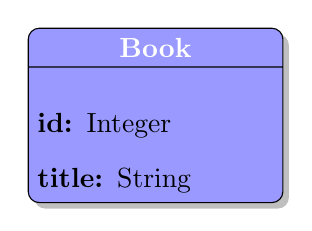
\begin{tikzpicture}
            \node (1)[abstract, rectangle split, rectangle split parts=2] at (4,8)
                {
                    \textbf{Book}
                    \nodepart{second} \begin{description}
                                          \item[id:] Integer
                                          \item[title:] String
                                      \end{description}
                };
        \end{tikzpicture}
    \caption{Graph mit 1 Type}
    \end{center}
    \label{fig:1type}
\end{figure}

Ein Objekt enthält 1 bis n Propertys. Diese Property kann entweder ein Standarddatentyp sein oder auf einen Type verweisen,
dies kann der eigene Type oder auch ein anderer Type sein.
Fügen wir unserem Beispiel des Buches eine Property hinzu mit dem Type Author wobei der Author selbst
wie folgt definiert wird:

\begin{center}
    \begin{verbatim}
        type Book {
            id: Int
            title: String
            author: Author
        }
        type Author {
            id: Int
            name: String
        }
    \end{verbatim}
\end{center}

So fügen wir unserem Graphen einen zusätzlichen Knoten hinzu
Die Beziehung zwischen dem Buch und Author wird durch eine gerichtete Kante zwischen dem Buch und dem Author dargestellt.
Hierdurch ergibt sich folgender Graph:

\begin{figure}
    \begin{center}
        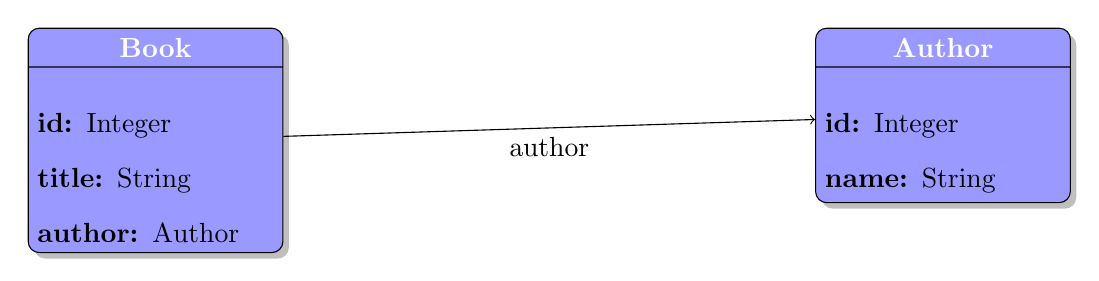
\begin{tikzpicture}
            \node (1)[abstract, rectangle split, rectangle split parts=2] at (0,0)
                {
                \textbf{Book}
                \nodepart{second} \begin{description}
                                      \item[id:] Integer
                                      \item[title:] String
                                      \item[author:] Author
                \end{description}
                };
            \node (2)[abstract, rectangle split, rectangle split parts=2] at (10,0)
                {
                \textbf{Author}
                \nodepart{second} \begin{description}
                                      \item[id:] Integer
                                      \item[name:] String
                \end{description}
                };
            \draw [->] (1) to node [midway,below]{author} (2);
        \end{tikzpicture}
    \end{center}
    \label{fig:2types}
\end{figure}

Fügen wir dem Author nun auch noch die Property written hinzu, so ergibt sich ein Kreis in diesem Graph.

\begin{verbatim}
    type Book {
        id: Int
        title: String
        author: Author
    }
    type Author {
        id: Int
        name: String
        written: [Books!]
    }
\end{verbatim}

so ergibt sich, dass wir einen zirkulären Graphen haben mit folgender Struktur

\begin{center}
    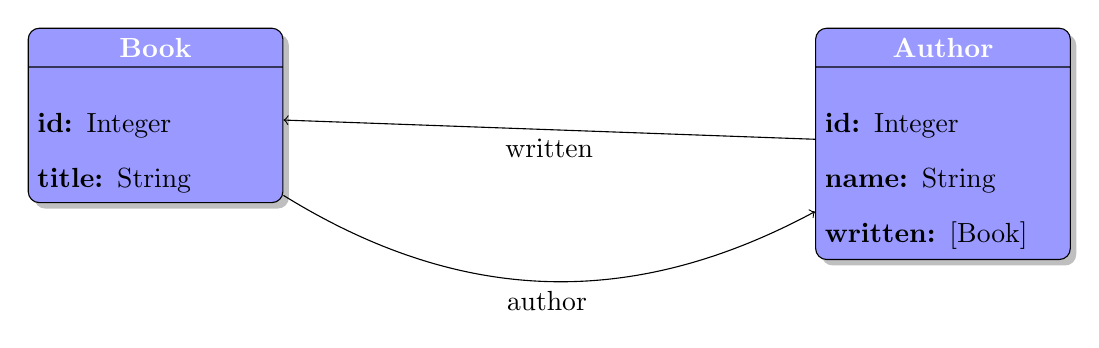
\begin{tikzpicture}
        \node (1)[abstract, rectangle split, rectangle split parts=2] at (0,0)
                {
                \textbf{Book}
                \nodepart{second} \begin{description}
                                      \item[id:] Integer
                                      \item[title:] String
                \end{description}
            };
            \node (2)[abstract, rectangle split, rectangle split parts=2] at (10,0)
                {
                \textbf{Author}
                \nodepart{second} \begin{description}
                                      \item[id:] Integer
                                      \item[name:] String
                                      \item[written:] [Book]
                \end{description}
            };

            \draw [ -> ] (1) to [bend right] node [midway,below]{ author } (2);
            \draw [ -> ] (2) to node [midway,below]{written} (1);
    \end{tikzpicture}
\end{center}


Dieses Schema ist ein Bauplan für einen sehr einfachen, zirkulären Graphen der durch GraphQL abgebildet wird.
In Realität können die Graphstrukturen die aus diesem Bauplan resultieren sehr unterschiedlich sein.
Für dieses Beispiel kann das bedeuten, dass folgende beide Graphen korrekt definierte Graphen sind jedoch komplett
andere Möglichkeiten bieten wie man sie abfragen kann. Hierdurch resultiert auch, dass die Abfragen
diverse Möglichkeiten haben je nach den unterliegenden Daten.

\begin{figure}
    \begin{center}
        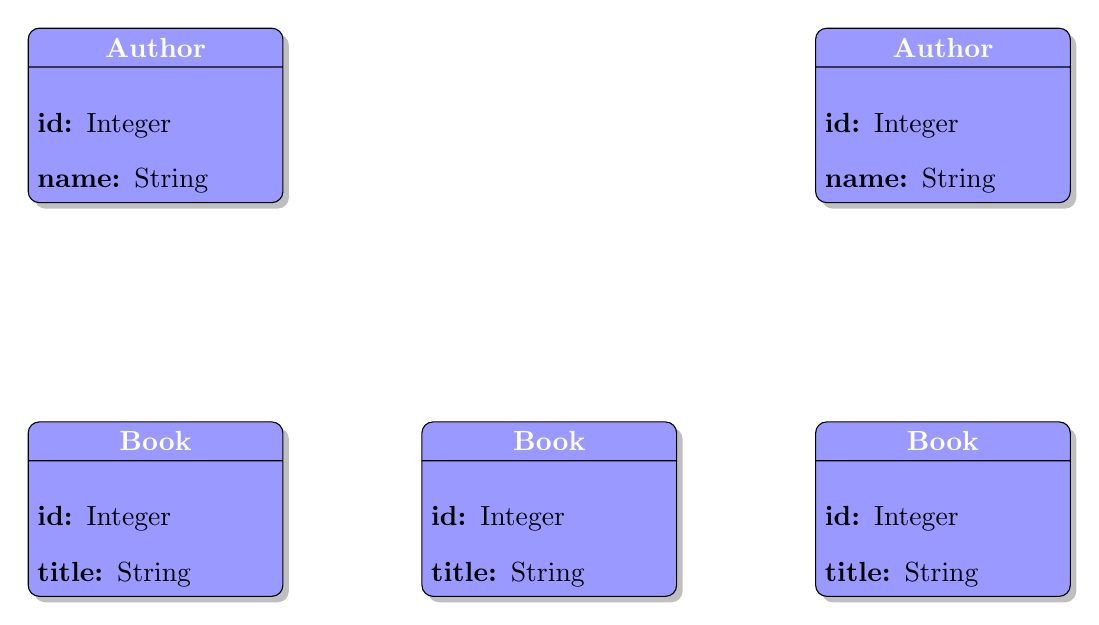
\begin{tikzpicture}
            \node (1)[abstract, rectangle split, rectangle split parts=2] at (0,0)
                {
                \textbf{Book}
                \nodepart{second} \begin{description}
                                      \item[id:] Integer
                                      \item[title:] String
                \end{description}
            };
            \node (2)[abstract, rectangle split, rectangle split parts=2] at (5,0)
                {
                \textbf{Book}
                \nodepart{second} \begin{description}
                                      \item[id:] Integer
                                      \item[title:] String
                \end{description}
            };
            \node (3)[abstract, rectangle split, rectangle split parts=2] at (10,0)
                {
                \textbf{Book}
                \nodepart{second} \begin{description}
                                      \item[id:] Integer
                                      \item[title:] String
                \end{description}
            };
            \node (4)[abstract, rectangle split, rectangle split parts=2] at (0,5)
                {
                \textbf{Author}
                \nodepart{second} \begin{description}
                                      \item[id:] Integer
                                      \item[name:] String
                \end{description}
            };
            \node (5)[abstract, rectangle split, rectangle split parts=2] at (10,5)
                {
                \textbf{Author}
                \nodepart{second} \begin{description}
                                      \item[id:] Integer
                                      \item[name:] String
                \end{description}
            };
        \end{tikzpicture}
    \caption{3 Bücher, 2 Autoren}
    \end{center}
\end{figure}


\begin{figure}
    \begin{center}
        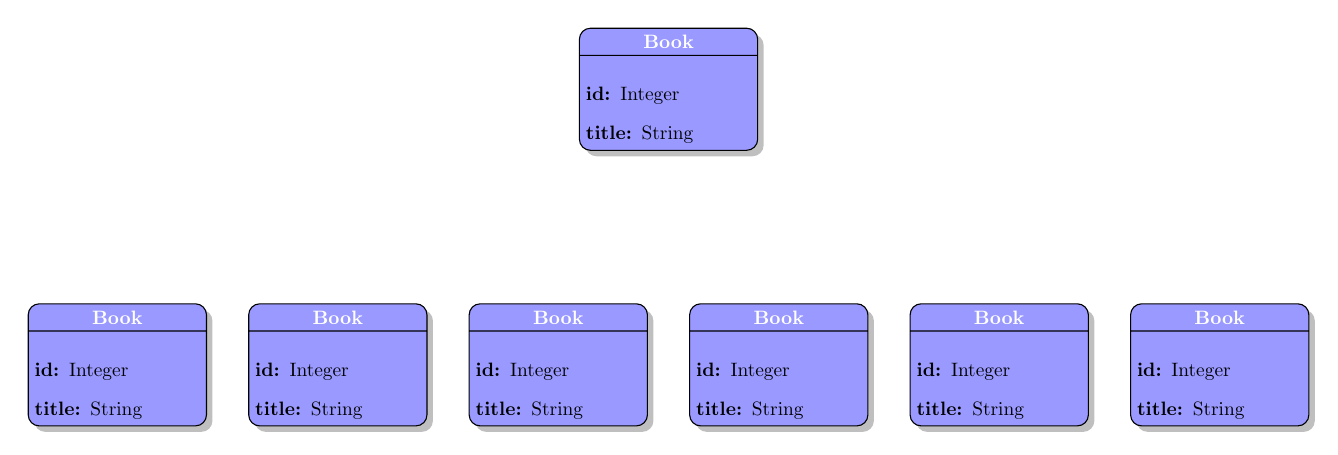
\begin{tikzpicture}[scale=0.7, transform shape]
            \node (1)[abstract, rectangle split, rectangle split parts=2] at (0,0)
                {
                \textbf{Book}
                \nodepart{second} \begin{description}
                                      \item[id:] Integer
                                      \item[title:] String
                \end{description}
            };
            \node (2)[abstract, rectangle split, rectangle split parts=2] at (4,0)
                {
                \textbf{Book}
                \nodepart{second} \begin{description}
                                      \item[id:] Integer
                                      \item[title:] String
                \end{description}
            };
            \node (3)[abstract, rectangle split, rectangle split parts=2] at (8,0)
                {
                \textbf{Book}
                \nodepart{second} \begin{description}
                                      \item[id:] Integer
                                      \item[title:] String
                \end{description}
            };
            \node (4)[abstract, rectangle split, rectangle split parts=2] at (12,0)
                {
                \textbf{Book}
                \nodepart{second} \begin{description}
                                      \item[id:] Integer
                                      \item[title:] String
                \end{description}
            };
            \node (5)[abstract, rectangle split, rectangle split parts=2] at (16,0)
                {
                \textbf{Book}
                \nodepart{second} \begin{description}
                                      \item[id:] Integer
                                      \item[title:] String
                \end{description}
            };
            \node (6)[abstract, rectangle split, rectangle split parts=2] at (20,0)
                {
                \textbf{Book}
                \nodepart{second} \begin{description}
                                      \item[id:] Integer
                                      \item[title:] String
                \end{description}
            };
            \node (7)[abstract, rectangle split, rectangle split parts=2] at (10,5)
                {
                \textbf{Book}
                \nodepart{second} \begin{description}
                                      \item[id:] Integer
                                      \item[title:] String
                \end{description}
            };
        \end{tikzpicture}
        \caption{6 Bücher, 1 Autor}
    \end{center}
\end{figure}

Definiert man nun, dass es zum Beispiel die StandardQuery "getBookAuthor(id): Author" geben soll. So bedeutet dies,
dass ein Author eines Buches abgefragt werden soll aufgrund der Id eines Buches.

(Hier Graphen einfügen mit Highlight der gewählten Knoten)




  \chapter{Praxis}

Nach der Einführung der Methode im vorherigen Kapitel soll nun der entwickelte Prototyp umfassend erklärt werden.
Der entwickelte Prototyp lässt sich unter \href{https://github.com/gernhard1337/graphql-primepath-tester} finden und testen.
Eine erklärende Readme existiert im Root-Verzeichnis.
Vorraussetzungen zum Ausführen der Anwendung ist Python und diverse Dritt-Bibliotheken die in der Readme vermerkt sind.

\section{Tool- / Dependencyauswahl}
Um die vorgestellte Methode umzusetzen war insbesondere wichtig, dass eine einfache und mächtige Bibliothek für die Definition und Bearbeitung
von Graphen zur Verfügung steht.
Die erste Wahl fiel hierbei auf NetworkX, eine Graphenbibliothek in Python.
Sie wurde ausgewählt da der Ersteller schon einige Erfahrungen mit dieser Bibliothek hat und somit eine effiziente Umsetzung möglich war.
Dadurch, dass diese Bibliothek als Grundlage gewählt wurde hat sich die Programmiersprache Python schnell ergeben.
Im folgenden werden einige weitere benutzte Bibliotheken kurz vorgestellt sodass der Applikationsstack übersichtlich wird.
Wir werden auch auf NetworkX und seine Features eingehen.
Es werden nicht alle Bibliotheken eine Berücksichtigung finden sondern nur diese, die einen signifikanten Einfluss auf das Programm haben und besonders herausstechen.

\subsection{NetworkX}

NetworkX ist eine Python-Biblitohek für \textit{Erstellung, Manipulation und Untersuchung der Struktur, Dynamik und Funktionen komplexer Netzwerke}~\cite[vgl. Startseite]{networkx}
Mit einer Star-Anzahl von \textit{12.8k}\cite{networkxgithub} auf GitHub ist networkX eine sehr beliebte Bibliothek.
NetworkX ist die ideale Wahl um Graphen zu erstellen für unseren Use-Case denn es nimmt jeden möglichen Datentypen als Wert für einen Knoten und Kante.
Wir können also sehr simpel Graphen definieren.
Für das simple Beispiel von Author, Book, Publisher und deren Verbindungen benötigen wir nur folgende Zeilen:

\begin{lstlisting}[language=Python]
    import networkx as nx

    G = nx.Graph()
    G.add_edge("Query", "Book", "book")
    G.add_edge("Query", "Author", "author")
    G.add_edge("Query", "Publisher", "publisher")

    G.add_edge("Publisher", "Book", "book")
    G.add_edge("Book", "Publisher", "publisher")

    G.add_edge("Book", "Author", "author")
    G.add_edge("Author", "Book", "book")
\end{lstlisting}

Diese wenigen Zeilen reichen aus um unseren Graphen mit allen Knoten und Kanten zu definieren.
Wie zuvor eingeführt existiert auch das Kantengewicht, dass der Feldbezeichner eines Types ist.
Auf diesem Graphen können wir dann diverse Algorithmen ablaufen lassen.
Diverse Hilfsfunktionen helfen dabei eine effiziente Programmierung zu erlangen.
Hierbei seien insbesondere folgende Hilfsfunktionen genannt:

\subsubsection{draw}
    \begin{lstlisting}[language=Python]
        nx.draw(G, with_labels=True)
    \end{lstlisting}

Zeichnet einem den erstellten Graphen in ein beliebiges Format.
So fällt es einfach große Graphen darzustellen.

\subsubsection{shortest\_path}
    \begin{lstlisting}[language=Python]
        shortest_path = nx.shortest_path(G, Node1, Node5)
    \end{lstlisting}

Die Funktion $shortest\_path$ gibt eine Liste von Kanten zurück, die den kürzesten Weg zwischen zwei
Knoten angibt.

\subsubsection{neighbors}
    \begin{lstlisting}[language=Python]
        G.neighbors(Node)
    \end{lstlisting}
Diese Funktion liefert alle Nachbarn eines Knotens.
In unserem Kontext eine sehr wichtige Funktion wie wir später noch sehen werden.

\subsection{Faker}
Die gewählte Datengenerierungsbibliothek ist \textit{Faker}\cite{fakergithub}.
Mit \textit{16k}\cite{fakergithub} Sternen auf GitHub ist Faker eine noch beliebtere Bilbiothek als NetworkX.
Faker ist eine Bilbiothek die es sehr einfach macht Daten zu generieren.
Da wir im Kontext von GraphQL Argumenten nur sehr einfache Datentypen als Argumente benötigen reicht uns diese
Bibliothek komplett aus da sie es schafft uns schnell und unkompliziert Daten in genau dem Format zu generieren wie wir sie brauchen.
Angenommen wir benötigen einen String der 10 Zeichen lang ist, so reicht eine Zeile:

\begin{lstlisting}[language=Python]
        random_string = fake.pystr(min_chars=10, max_chars=10)
\end{lstlisting}

Selbiges falls wir eine Zufallszahl benötigen zwischen 1 bis 1000

\begin{lstlisting}[language=Python]
        random_number = fake.random_int(min=1, max=1000)
\end{lstlisting}

Diese Schema des Einzeilers zieht sich für alle simplen $SCALAR$ Types in GraphQL.
Daher fällt die Wahl für die Datengenerierung auf diese Bibliothek.

\subsection{PyTest}

Nicht zwingend notwendig ist ein Testframework.
Allerdings soll unsere Implementation der Methode Tests erstellen sodass diese zu einem späteren Zeitpunk erneut ausgeführt werden können.
Somit können wir z.B. überprüfen ob eine Korrektur des Servercodes eine Verbesserung gebracht hat.
Hierfür wollen wir die Tests mithilfe eines Testframeworks erstellen.
Die Wahl hierfür fiel dabei auf PyTest.
PyTest ist ein Testframework für Python welches eine simple und einfache Testdefinition ermöglicht.
Ein Test für eine einfache Funktion $inc$ kann mit $test\_inc$ umgesetzt werden.

\begin{lstlisting}[language=Python]
    def inc(x):
        return x + 1

    def test_inc():
        assert inc(3) == 5
\end{lstlisting}

Dies reicht schon vollkommen aus für unsere Testentwicklung daher wurde sich für diese Bibliothek entschieden.

\section{Umsetzung der Methode}

Für die Umsetzung der Methode werden wir durch die einzelnen Teile des Codes gehen und die jeweiligen Stellen erklären die
einzelne Schritte der entwickelten Methode durchgehen.
Hierbei gehen wir chronologisch in den einzelnen Schritten vor so wie in der Methode definiert.

\subsection{Schema in Graph abbilden}

Wie in der Vorstellung der Methode unter $6.1$ bilden wir das GraphQL-Schema in einem Graphen ab.
Hierfür nutzen wir die zuvor erwähnt Python Graphbibliothek NetworkX.
Um die Informationen zu erlangen die für die Bildung des Graphens wichtig sind führen wir die Introspection-Query \ref{introspection-query}
aus.
Das Ergebnis ist dann das vollständige GraphQL-Schema der API.
Hierbei sei angemerkt, dass einige GraphQL APIs so eine Introspection-Query verbieten, sei es einerseits durch direktes verbieten oder ein Tiefenlimit in den Querys.
Egal was hierbei der Fall ist, die zu testende API muss unsere Introspection-Query \ref{introspection-query} unterstützen.
Die Query wird mit einem simplen HTTP-POST an die zu testende URL gesendet.

\begin{lstlisting}[language=Python]
    r = requests.post(testUrl, json={'query': queries.introspection_query})
    json_data = json.loads(r.text)
    with open('schema.json', 'w') as f:
        json.dump(json_data, f)
\end{lstlisting}

Und die Response wird als JSON-Objekt in $json\_data$ gespeichert.
Zudem speichern wir das JSON-Objekt der aktuellen API auch ab damit diese später gegebenenfalls untersucht werden kann.
Es wurde ein Modul $Graphhandler$ entwickelt, dass verschiedene Graphoperationen für einen Übernimmt.
Im Graphhandler ist eine Funktion $buildGraph$ definiert.
Diese generiert einen Graphen von einem gegebenen Startknoten, einem leeren Graphen und dem Schema.
Hierbei werden nur erreichbare Knoten von Startknoten berücksichtigt.
Setzt man den Startknoten auf den Knoten $Query$ so inkludieren wir auf diese Weise nur alle erreichbaren Teile
des Graphens ausgehend von $Query$.
Dies ist insofern sinnvoll da andere Typen, wenn sie nicht von $Query$ aus erreichbar sind, nicht Teil des Testraumes wären da diese
in keiner validen Anfrage vorkommen können.
Die Funktion, die den Graphen generiert sieht wie folgt aus:

\begin{lstlisting}[language=Python]
def buildGraph(graph, type_name, type_dict):
    if type_name.startswith(nonSchemaTypePrefix) or type_name in baseDatatypes:
        pass
    else:
        for adjacentNode in type_dict[type_name]['fields']:
            if graph.has_edge(type_name, adjacentNode['type']['name']):
                return
            else:
                if adjacentNode['type']['name'] and adjacentNode['type']['name'] not in baseDatatypes:
                    graph.add_edge(type_name, adjacentNode['type']['name'])
                    graph[type_name][adjacentNode['type']['name']]["data"] = adjacentNode
                    buildGraph(graph, adjacentNode['type']['name'], type_dict)
                if adjacentNode['type']['kind'] == 'LIST' and adjacentNode['type']['ofType']['name'] not in baseDatatypes:
                    graph.add_edge(type_name, adjacentNode['type']['ofType']['name'])
                    graph[type_name][adjacentNode['type']['ofType']['name']]["data"] = adjacentNode
                    buildGraph(graph, adjacentNode['type']['ofType']['name'], type_dict)

\end{lstlisting}

Die Funktion buildGraph arbeitet rekursiv.
Vom Startknoten (im Allgemeinen $Query$) aus rufen wir die Funktion auf allen Folgeknoten von Query auf.
Dies sind alle Knoten die den Type $OBJECT$ besitzen und nicht mit einem $\_\_$ beginnen oder ein Basisdatentyp sind.
GraphQL kann eigene Objekte definieren welche mit $\_\_$ starten, diese schließen wir explizit aus genau wie alle $SCALAR$ Types.
Jeder Knoten definiert nun in seinem $fields$ Eintrag zu welchen Feldern er Beziehungen hat.
Hierbei muss unterschieden werden, dass ein Eintrag entweder vom Type $OBJECT$ oder $LIST$ sein kann, um zulässig zu sein.
Sollte es sich um einen $LIST$ Eintrag handeln müssen wir prüfen von welchem Type die $LIST$ ist.
Wenn ein Knoten nun unsere Bedingungen erfüllt, so wird dieser dem Graphen hinzugefügt und auf ihm selbst wird $buildGraph$ ausgeführt.
So erlangen wir die gesamte Graphstruktur da ausgehend von Query jeder erreichbare Knoten hinzugefügt wird und dann von diesem Knoten eben wieder alle erreichbaren Knoten
hinzugefügt werden.

\subsection{Pfade aus Graph bilden}

Der Graphhandler implementiert verschiedene Coveragekriterien.
Das Tool benötigt eine Liste $paths$ die aus Kanten besteht.

\begin{lstlisting}[language=Python]
paths = graphhandler.generate_prime_paths("Query", graph)
\end{lstlisting}

Eine Funktion $generate\_CoverPaths$ kann jedes erdenkliche Coveragekriterium umsetzen.
In unserem Fall sind es insbesondere PrimePaths, umgesetzt durch die Funktion $generare\_prime\_paths("Query", graph)$.
Diese Funktion ermittelt die PrimePaths ausgehend vom Startknoten $Query$ im definierten Graphen.
Will man ein anderes Coveragekriterium umsetzen, so muss die Funktion $generate\_CoverPaths$ eine Liste der Kanten zurückgeben
die dem Coveragekriterium entsprechend den Graphen überdecken.
Die Generierung der PrimePaths sehen wir uns nun noch genauer an.
Wir starten mit der Funktion $generare\_prime\_paths()$.
Diese bekommt einen Startknoten und einen Graphen.
Sie gibt dann die Liste der Pfade genau wie zuvor spezifiziert zurück.

\begin{lstlisting}[language=Python]
def generate_prime_paths(startknoten, g):
    pfadliste = []
    generate_paths(startknoten, [], pfadliste, g)
    return pfadliste
\end{lstlisting}

Es wird die Funktion $generate\_paths$ aufgerufen wobei generate\_paths sich immer wieder rekursiv selbst aufruft wenn die Nachfolger des Knotens
noch nicht im Pfad sind. So werden Kreise verhindert, alle Pfade die so erzeugt werden sind SimplePaths.

\begin{lstlisting}[language=Python]
def generate_paths(n, path, pathList, g):
    path.append(n)
    for m in g.successors(n):  # successors gibt die Nachfolger wieder
        if m not in path:
            generate_paths(m, copy.deepcopy(path), pathList, g)
    if is_prime_path(path, pathList):
        pathList.append(path)
\end{lstlisting}

Sollte ein SimplePath dann ein PrimePath sein so wird dieser zurückgegeben.
Ein Pfad ist ein Prime-Pfad, wenn er kein Teil eines bereits existierenden Pfades ist und keine Kreise enthält.
Diese drei hier vorgestellten Funktionen setzen den Pseudocode aus $6.3.2$ um

\begin{lstlisting}[language=Python]
def is_prime_path(new_path, pathList):
    for exisiting_paths in pathList:
        if is_subpath(new_path, exisiting_paths):
            return False
    return True
\end{lstlisting}





% Das wird in der Implementierung teilweise schon anders gemacht und wird vielleicht nicht gebraucht.
\subsection{Coveragepfade ermitteln (maybe remove - TODO)}


\subsection{Querys aus Pfad ermitteln}
\subsection{Test ausführen / Testfile generieren}
\subsection{Testauswertung}

\newpage
\section{Zusammenfassung der Implementation}

Die entwickelte Methode lässt sich in folgendem Sequenzdiagramm gut abbilden:

\begin{center}
    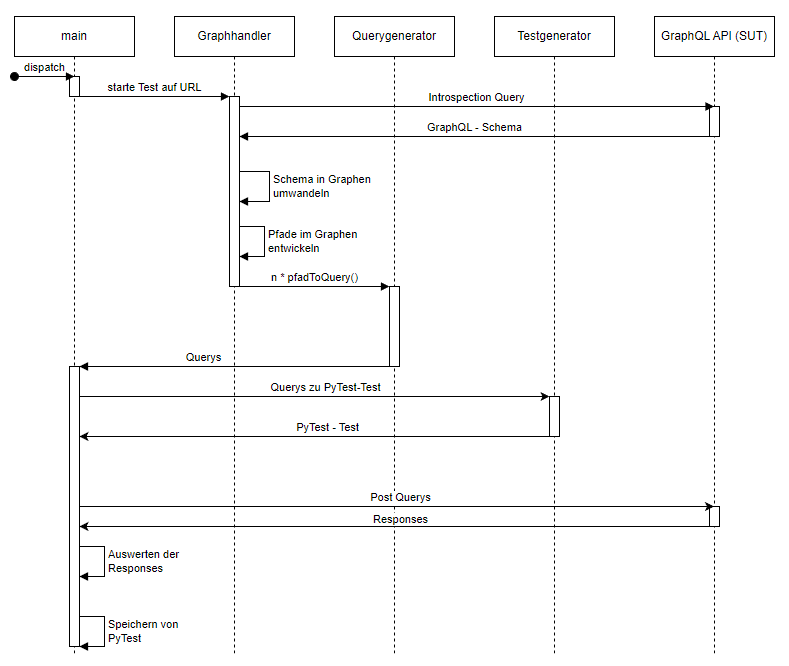
\includegraphics[width=\textwidth,height=\textheight,keepaspectratio]{img/sequenz}
\end{center}








  \backmatter % kennzeichnet den hinteren Teil der Arbeit
  %! Author = Tom
\chapter{Glossar}

Im Text werden einige Fachbegriffe genutzt. Hier findet sich deren Erklärung

\begin{description}
    \item[Begriff] Erklärung
    \item[IEEE/ACM] Ein Journal über Transaktionen in Netzwerken das regelmäßig Konferenzen veranstaltet
    \item[HTTP] HyperTextTransferProtocoll ist ein Übertragunsprotokoll für Datenübertragung
    \item[HTTP-Request] Ist eine Anfrage zum zusenden von Daten
    \item[API] Application Programmable Interface ist eine Schnittstelle wie Systeme miteinander kommunizieren
    \item[REST] Ein Architekturdesign für APIs
    \item[GraphQL] Eine Abfragesprache für APIs die den GraphQL Standard implementieren
    \item[Overfetch] Das Abfrgaen von zu vielen Informationen
    \item[Underfetch] Das Abfragen von zu wenigen Informationen
    \item[SUT] System under Test - ist eine Kurzform für das System, dass es zu testen gilt
    \item[IoT] Internet of Things - meint die Verknüpfung von diversen Geräten mit dem Internet
\end{description}


  \appendix % Anhang

  \cleardoublepage
  \addcontentsline{toc}{chapter}{Literaturverzeichnis}
  % \nocite{*}  % Hier das Kommentarzeichen entfernen, um alle Quellen auszugeben.
  \printbibliography[title={Literaturverzeichnis}]  % Generiert das Literaturverzeichnis

  \vfill
  \begin{center}
   \emph{Onlineressourcen wurden im Juli 2021 auf ihre Verfügbarkeit hin überprüft.}
  \end{center}

\end{document}
